% !TeX root = ../Book1.tex
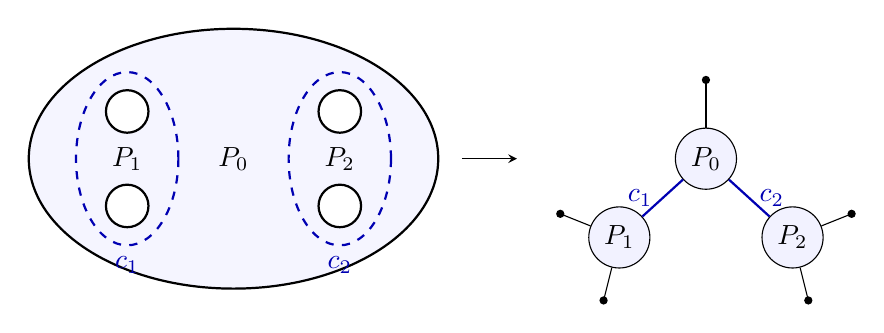
\begin{tikzpicture}[x=1cm,y=1cm,>=stealth]
	\draw[thick,fill=blue!4] (0,0) ellipse (2.6 and 1.65);
	\foreach \x in {-1.35,1.35}{
		\draw[thick,fill=white] (\x,0.6) circle (0.27);
		\draw[thick,fill=white] (\x,-0.6) circle (0.27);
		\draw[blue!70!black,thick,dashed] (\x,0) ellipse (0.65 and 1.1);
	}
	\node at (0,0) {\(P_0\)};
	\node at (-1.35,0) {\(P_1\)};
	\node at (1.35,0) {\(P_2\)};
	\node[blue!70!black] at (-1.35,-1.35) {\(c_1\)};
	\node[blue!70!black] at (1.35,-1.35) {\(c_2\)};
	\draw[->] (2.9,0)--(3.6,0);
	\begin{scope}[shift={(6,0)}]
		\node[circle,draw,fill=blue!5,inner sep=3pt] (p0) at (0,0) {\(P_0\)};
		\node[circle,draw,fill=blue!5,inner sep=3pt] (p1) at (-1.1,-1) {\(P_1\)};
		\node[circle,draw,fill=blue!5,inner sep=3pt] (p2) at (1.1,-1) {\(P_2\)};
		\draw[blue!70!black,thick] (p0)--node[left] {\(c_1\)}(p1);
		\draw[blue!70!black,thick] (p0)--node[right] {\(c_2\)}(p2);
		\draw (p0)--(0,1);
		\draw (p1)--(-1.85,-0.7);
		\draw (p1)--(-1.3,-1.8);
		\draw (p2)--(1.85,-0.7);
		\draw (p2)--(1.3,-1.8);
		\foreach \x/\y in {0/1,-1.85/-0.7,-1.3/-1.8,1.85/-0.7,1.3/-1.8}{
			\fill (\x,\y) circle (1.5pt);
		}
	\end{scope}
\end{tikzpicture}
